\documentclass{standalone}
\usepackage{tikz}
\usetikzlibrary{patterns, positioning}
\usetikzlibrary{shapes.misc}
\usepackage[outline]{contour}
\contourlength{1.5pt} 
\usepackage[sfdefault]{ClearSans} %% option 'sfdefault' activates Clear Sans as the default text font
\usepackage[T1]{fontenc}

\begin{document}
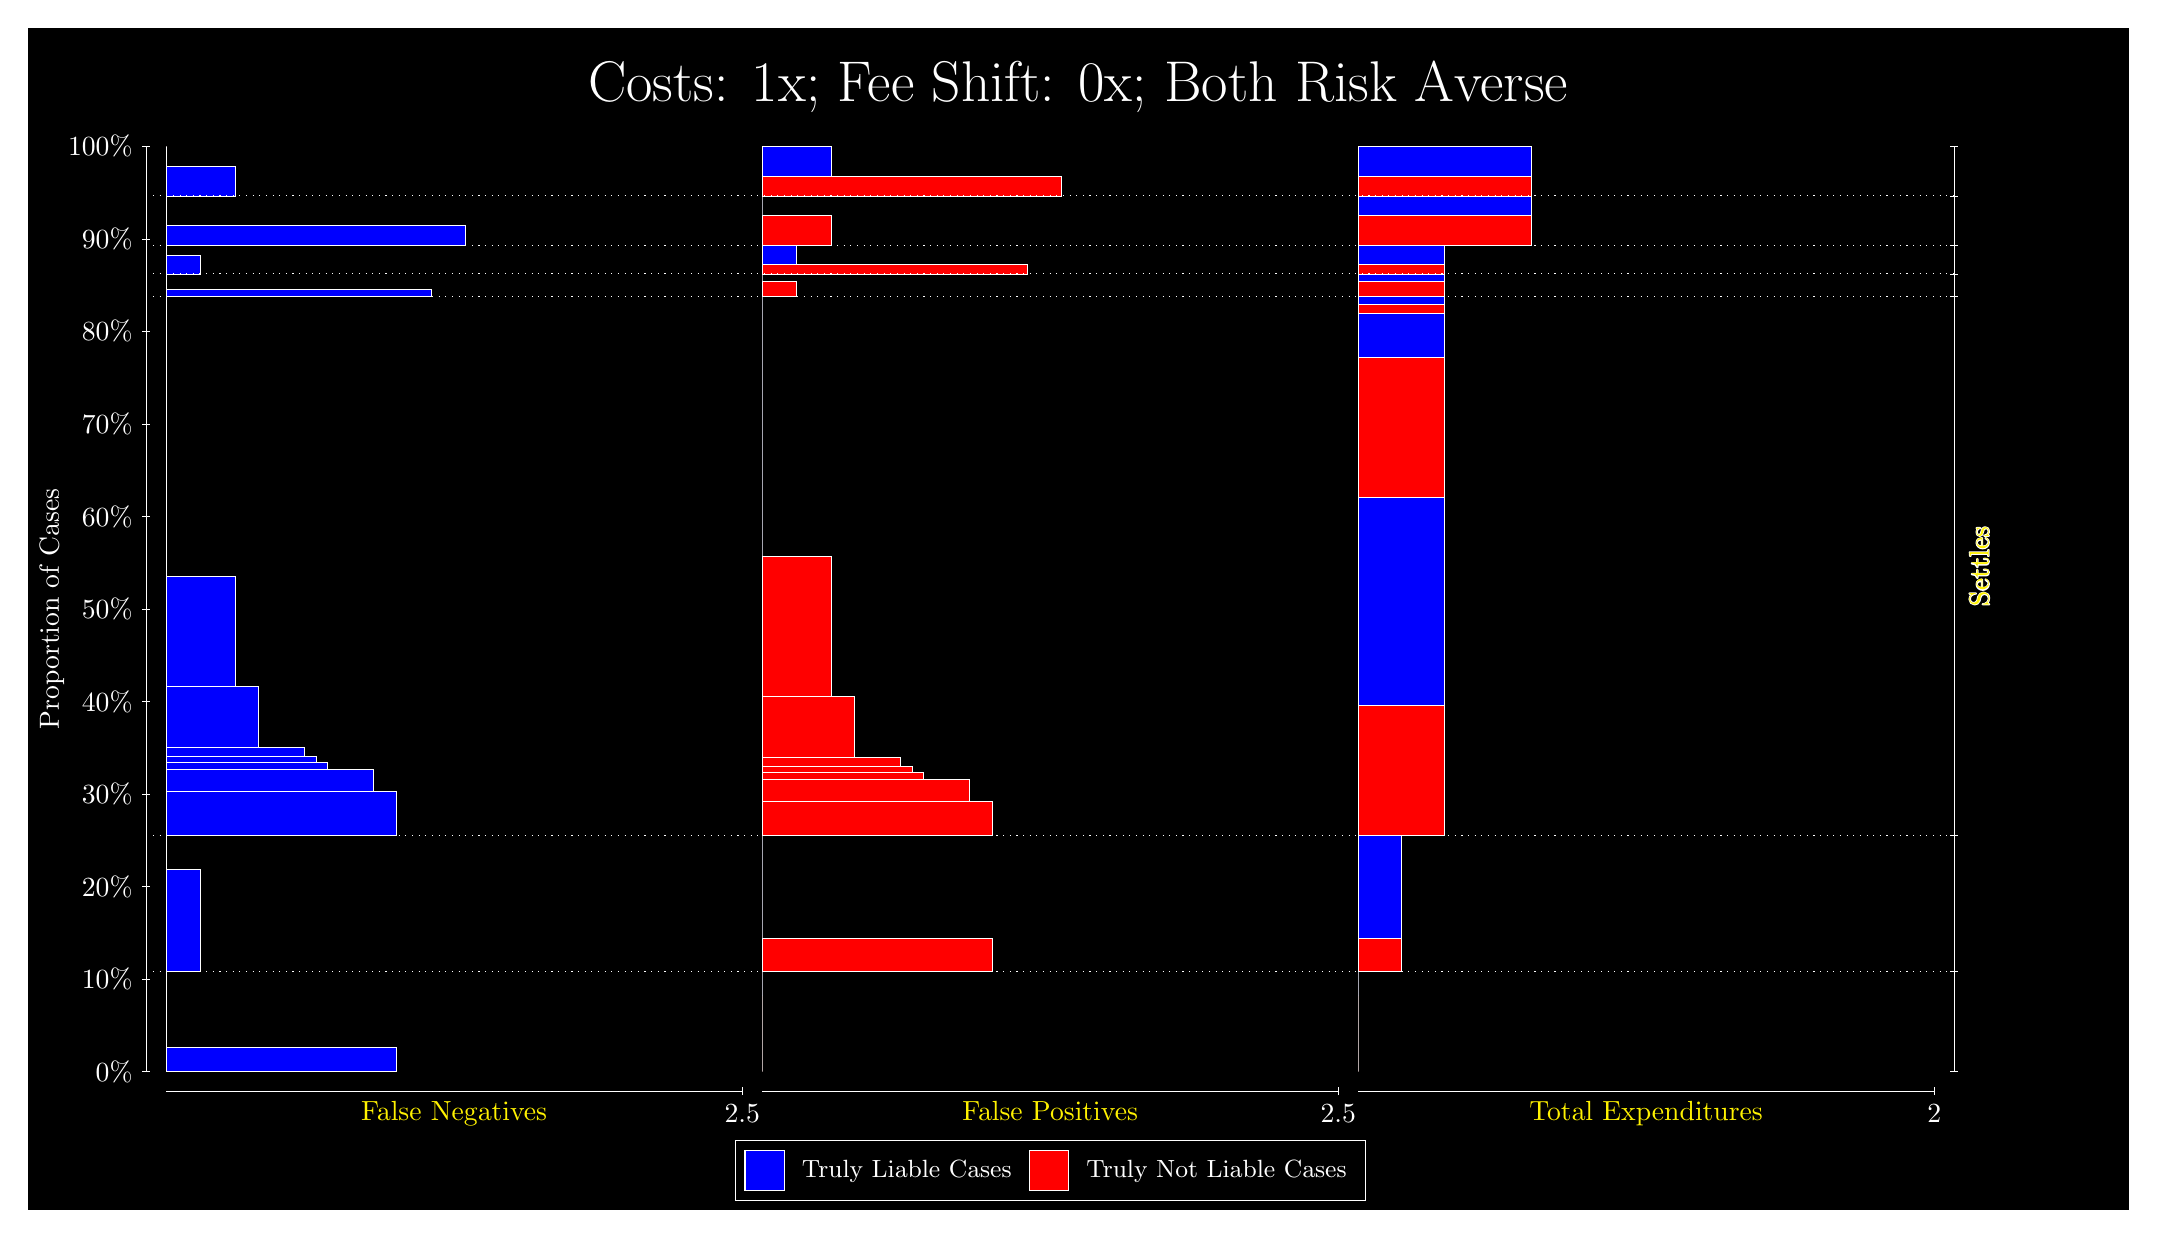
\begin{tikzpicture}
\draw[fill=black] (0,0) rectangle (26.667,15);
\draw[text=white] (0,13.5) rectangle (26.667,15) node[midway] {\huge Costs: 1x; Fee Shift: 0x; Both Risk Averse};
\draw[white, very thin] (1.5,1.75) -- (1.5,13.5);
\node[rotate=90, text=white, anchor=center] at (0.3, 7.625) {Proportion of Cases};
\draw[white, very thin] (1.45,1.75) -- (1.55,1.75);
\node[text=white, anchor=east] at (1.45, 1.75) {0\%};
\draw[white, very thin] (1.45,2.925) -- (1.55,2.925);
\node[text=white, anchor=east] at (1.45, 2.925) {10\%};
\draw[white, very thin] (1.45,4.1) -- (1.55,4.1);
\node[text=white, anchor=east] at (1.45, 4.1) {20\%};
\draw[white, very thin] (1.45,5.275) -- (1.55,5.275);
\node[text=white, anchor=east] at (1.45, 5.275) {30\%};
\draw[white, very thin] (1.45,6.45) -- (1.55,6.45);
\node[text=white, anchor=east] at (1.45, 6.45) {40\%};
\draw[white, very thin] (1.45,7.625) -- (1.55,7.625);
\node[text=white, anchor=east] at (1.45, 7.625) {50\%};
\draw[white, very thin] (1.45,8.8) -- (1.55,8.8);
\node[text=white, anchor=east] at (1.45, 8.8) {60\%};
\draw[white, very thin] (1.45,9.975) -- (1.55,9.975);
\node[text=white, anchor=east] at (1.45, 9.975) {70\%};
\draw[white, very thin] (1.45,11.15) -- (1.55,11.15);
\node[text=white, anchor=east] at (1.45, 11.15) {80\%};
\draw[white, very thin] (1.45,12.325) -- (1.55,12.325);
\node[text=white, anchor=east] at (1.45, 12.325) {90\%};
\draw[white, very thin] (1.45,13.5) -- (1.55,13.5);
\node[text=white, anchor=east] at (1.45, 13.5) {100\%};

\draw[white, very thin] (24.457,1.75) -- (24.457,13.5);
\draw[white, very thin] (24.407,1.75) -- (24.507,1.75);
\node[anchor=west] at (24.407, 1.75) {};
\draw[white, very thin] (24.407,3.0175) -- (24.507,3.0175);
\node[anchor=west] at (24.407, 3.0175) {};
\draw[white, very thin] (24.407,4.7461) -- (24.507,4.7461);
\node[anchor=west] at (24.407, 4.7461) {};
\draw[white, very thin] (24.407,11.59) -- (24.507,11.59);
\node[anchor=west] at (24.407, 11.59) {};
\draw[white, very thin] (24.407,11.88) -- (24.507,11.88);
\node[anchor=west] at (24.407, 11.88) {};
\draw[white, very thin] (24.407,12.241) -- (24.507,12.241);
\node[anchor=west] at (24.407, 12.241) {};
\draw[white, very thin] (24.407,12.871) -- (24.507,12.871);
\node[anchor=west] at (24.407, 12.871) {};
\draw[white, very thin] (24.407,13.5) -- (24.507,13.5);
\node[anchor=west] at (24.407, 13.5) {};

\draw[white, very thin, fill=blue] (1.75,1.75) rectangle (4.6775,2.0578);
\draw[white, very thin, fill=red] (1.75,2.0578) rectangle (1.75,3.0175);
\draw[white, very thin, fill=blue] (1.75,3.0175) rectangle (2.1891,4.3222);
\draw[white, very thin, fill=red] (1.75,4.3222) rectangle (1.75,4.7461);
\draw[white, very thin, fill=blue] (1.75,4.7461) rectangle (4.6775,5.3037);
\draw[white, very thin, fill=blue] (1.75,5.3037) rectangle (4.3848,5.5828);
\draw[white, very thin, fill=blue] (1.75,5.5828) rectangle (3.7993,5.6777);
\draw[white, very thin, fill=blue] (1.75,5.6777) rectangle (3.6529,5.7474);
\draw[white, very thin, fill=blue] (1.75,5.7474) rectangle (3.5065,5.8644);
\draw[white, very thin, fill=blue] (1.75,5.8644) rectangle (2.921,6.6469);
\draw[white, very thin, fill=blue] (1.75,6.6469) rectangle (2.6283,8.0427);
\draw[white, very thin, fill=red] (1.75,8.0427) rectangle (1.75,11.59);
\draw[white, very thin, fill=blue] (1.75,11.59) rectangle (5.1167,11.685);
\draw[white, very thin, fill=red] (1.75,11.685) rectangle (1.75,11.88);
\draw[white, very thin, fill=blue] (1.75,11.88) rectangle (2.1891,12.122);
\draw[white, very thin, fill=red] (1.75,12.122) rectangle (1.75,12.241);
\draw[white, very thin, fill=blue] (1.75,12.241) rectangle (5.5558,12.492);
\draw[white, very thin, fill=red] (1.75,12.492) rectangle (1.75,12.871);
\draw[white, very thin, fill=blue] (1.75,12.871) rectangle (2.6283,13.249);
\draw[white, very thin, fill=red] (1.75,13.249) rectangle (1.75,13.5);
\draw[white, very thin, fill=red] (9.3189,1.75) rectangle (9.3189,2.7097);
\draw[white, very thin, fill=blue] (9.3189,2.7097) rectangle (9.3189,3.0175);
\draw[white, very thin, fill=red] (9.3189,3.0175) rectangle (12.246,3.4414);
\draw[white, very thin, fill=blue] (9.3189,3.4414) rectangle (9.3189,4.7461);
\draw[white, very thin, fill=red] (9.3189,4.7461) rectangle (12.246,5.1781);
\draw[white, very thin, fill=red] (9.3189,5.1781) rectangle (11.954,5.4572);
\draw[white, very thin, fill=red] (9.3189,5.4572) rectangle (11.368,5.552);
\draw[white, very thin, fill=red] (9.3189,5.552) rectangle (11.222,5.6218);
\draw[white, very thin, fill=red] (9.3189,5.6218) rectangle (11.075,5.7388);
\draw[white, very thin, fill=red] (9.3189,5.7388) rectangle (10.49,6.5213);
\draw[white, very thin, fill=red] (9.3189,6.5213) rectangle (10.197,8.2938);
\draw[white, very thin, fill=blue] (9.3189,8.2938) rectangle (9.3189,11.59);
\draw[white, very thin, fill=red] (9.3189,11.59) rectangle (9.758,11.785);
\draw[white, very thin, fill=blue] (9.3189,11.785) rectangle (9.3189,11.88);
\draw[white, very thin, fill=red] (9.3189,11.88) rectangle (12.686,11.999);
\draw[white, very thin, fill=blue] (9.3189,11.999) rectangle (9.758,12.241);
\draw[white, very thin, fill=red] (9.3189,12.241) rectangle (10.197,12.62);
\draw[white, very thin, fill=blue] (9.3189,12.62) rectangle (9.3189,12.871);
\draw[white, very thin, fill=red] (9.3189,12.871) rectangle (13.125,13.121);
\draw[white, very thin, fill=blue] (9.3189,13.121) rectangle (10.197,13.5);
\draw[white, very thin, fill=red] (16.888,1.75) rectangle (16.888,2.7097);
\draw[white, very thin, fill=blue] (16.888,2.7097) rectangle (16.888,3.0175);
\draw[white, very thin, fill=red] (16.888,3.0175) rectangle (17.437,3.4414);
\draw[white, very thin, fill=blue] (16.888,3.4414) rectangle (17.437,4.7461);
\draw[white, very thin, fill=red] (16.888,4.7461) rectangle (17.986,6.4044);
\draw[white, very thin, fill=blue] (16.888,6.4044) rectangle (17.986,9.0485);
\draw[white, very thin, fill=red] (16.888,9.0485) rectangle (17.986,10.821);
\draw[white, very thin, fill=blue] (16.888,10.821) rectangle (17.986,11.379);
\draw[white, very thin, fill=red] (16.888,11.379) rectangle (17.986,11.496);
\draw[white, very thin, fill=blue] (16.888,11.496) rectangle (17.986,11.59);
\draw[white, very thin, fill=red] (16.888,11.59) rectangle (17.986,11.785);
\draw[white, very thin, fill=blue] (16.888,11.785) rectangle (17.986,11.88);
\draw[white, very thin, fill=red] (16.888,11.88) rectangle (17.986,11.999);
\draw[white, very thin, fill=blue] (16.888,11.999) rectangle (17.986,12.241);
\draw[white, very thin, fill=red] (16.888,12.241) rectangle (19.083,12.62);
\draw[white, very thin, fill=blue] (16.888,12.62) rectangle (19.083,12.871);
\draw[white, very thin, fill=red] (16.888,12.871) rectangle (19.083,13.121);
\draw[white, very thin, fill=blue] (16.888,13.121) rectangle (19.083,13.5);
\draw[white, dotted] (1.5,3.0175) -- (24.457,3.0175);
\draw[white, dotted] (1.5,4.7461) -- (24.457,4.7461);
\draw[white, dotted] (1.5,11.59) -- (24.457,11.59);
\draw[white, dotted] (1.5,11.88) -- (24.457,11.88);
\draw[white, dotted] (1.5,12.241) -- (24.457,12.241);
\draw[white, dotted] (1.5,12.871) -- (24.457,12.871);
\draw[white, very thin] (1.75,1.5) -- (9.0689,1.5);
\node[text=yellow, anchor=north] at (5.4094, 1.5) {False Negatives};
\draw[white, very thin] (9.0689,1.45) -- (9.0689,1.55);
\node[text=white, anchor=north] at (9.0689, 1.45) {2.5};

\draw[white, very thin] (9.3189,1.5) -- (16.638,1.5);
\node[text=yellow, anchor=north] at (12.978, 1.5) {False Positives};
\draw[white, very thin] (16.638,1.45) -- (16.638,1.55);
\node[text=white, anchor=north] at (16.638, 1.45) {2.5};

\draw[white, very thin] (16.888,1.5) -- (24.207,1.5);
\node[text=yellow, anchor=north] at (20.547, 1.5) {Total Expenditures};
\draw[white, very thin] (24.207,1.45) -- (24.207,1.55);
\node[text=white, anchor=north] at (24.207, 1.45) {2};



\node[text=yellow, centered, rotate=90] at (24.777, 8.1682) {\contour{white}{Settles}};





\draw (12.978300999999998,1.5) node[draw=none] (baseCoordinate) {};
\begin{scope}[align=center]
        \matrix[scale=0.5, draw=white, below=0.5cm of baseCoordinate, nodes={draw}, column sep=0.1cm]{
            \node[rectangle, draw, minimum width=0.5cm, minimum height=0.5cm, fill=blue] {}; &
            \node[draw=none, font=\small, text=white] (B) {Truly Liable Cases}; &
            \node[rectangle, draw, minimum width=0.5cm, minimum height=0.5cm, fill=red] {}; &
            \node[draw=none, font=\small, text=white] (B) {Truly Not Liable Cases}; \\
            };
\end{scope}

\end{tikzpicture}
\end{document}